\documentclass{beamer}% This is the file main.tex
\usepackage{graphicx}
\usepackage{outlines}

\usetheme{Berlin}
\title{Introduction to Mechatronics Terms}
\author{Thad Hughes}
\date{\today}
\begin{document}

\maketitle

\begin{frame}
\frametitle{Outline}
\framesubtitle{Where are we going today?}

\begin{itemize}
	\item Mass
	\item Acceleration/Velocity
	\item Force
	\item Torque
	\item Work/Power/Energy
\end{itemize}

\begin{block}
	This may or may not be physics review for you. If it is, skim through, make sure you're comfy. If not, let this be a fun first foray!
\end{block}

\end{frame}



\begin{frame}
\frametitle{Mass}
\framesubtitle{Sitting around like a bump on a log}

\begin{outline}
	\1 Mass is "how much stuff is there?"
	\1 Not weight, but we commonly correlate the two on earth
		\2 (ignoring buoyancy) things of the same mass weigh the same in a constant gravitational field
\end{outline}

\begin{examples}
\begin{outline}
	\1 Kilograms (kg)
	\1 Slugs (slug)
	\1 Pounds-mass (lbm)
\end{outline}
\end{examples}

\begin{alertblock}{Warning}
	Pounds-Mass is not the same unit as Pounds-Force!
\end{alertblock}

\end{frame}


\begin{frame}
\frametitle{Velocity and Speed}
\framesubtitle{Gotta go Fast!}

\begin{outline}
	\1 Speed is how fast something is going- a scalar quantity
		\2 Scalar quantity
		\2 "Travelled 60 miles in one hour"
	\1 Velocity is how fast something is going in a direction
		\2 Vector quantity
		\2 "Travelling 30 MPH, Northeast"
\end{outline}

\begin{examples}
\begin{outline}
	\1 Miles per Hour (mph)
	\1 Meters per Second (m/s)
\end{outline}
\end{examples}

\begin{alertblock}{Warning}
	Rotational speed / velocity are different quantities. We'll get there!
\end{alertblock}

\end{frame}


\begin{frame}
\frametitle{Acceleration}
\framesubtitle{A thrill better than speed!}

Acceleration is how fast your velocity is changing.

If you accelerate from 30 ft/s to 10 ft/s in 4 s, that's
\begin{equation}
	a = \frac{\Delta v}{\Delta t} = \frac{10 \ \mbox{ft/s} - 30 \ \mbox{ft/s}}{4 s} = - 5 \frac{ft}{s^2} \nonumber
\end{equation} 
\begin{columns}
\column{0.5\textwidth}
Note: direction matters! You can have acceleration perpindicular to your movement. In the case of circular motion, this is known as centripetal acceleration. The tread of a spinning tire is always accelerating inwards.

\column{0.5\textwidth}
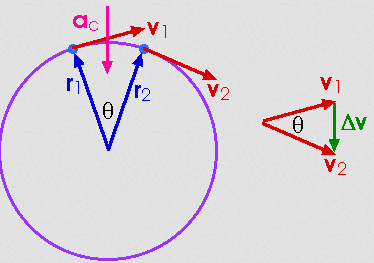
\includegraphics[width=1.0\textwidth]{img_Mechatronics_Terminology_centrip.png}
\end{columns}

\end{frame}

\begin{frame}
\frametitle{Force}
\framesubtitle{May the rate of change of momentum for a closed system be with you.}

A long while ago, this fellow Newton had an idea: what if objects interacted with each other via forces?
Turns out, it's at least a really good model.

\begin{columns}
\column{0.5\textwidth}
\begin{block}{Principle 1 - Proportionality}
	The net force on an object causes acceleration inversely proportional to its mass.
	\begin{equation}
		\sum \vec{F} = m \vec{a}
	\end{equation}
\end{block}

\column{0.5\textwidth}
\begin{block}{Principle 2 - Reciprocity}
	When a force is imposed upon object A by B, B sees a force of equal magnitude and opposite direction.
	\begin{equation}
		[\sum \vec{F}]_{universe} = 0
	\end{equation}
\end{block}

\end{columns}

\end{frame}

\end{document}